%%%%%%%%%%%%%%%%%%%%%%%%%%%%%%%%%%%%%%%%%%%%%%%%%%%%%%%%%%%%%%%%%%%%%%%%
% Plantilla TFG/TFM
% Escuela Politécnica Superior de la Universidad de Alicante
% Realizado por: Jose Manuel Requena Plens
% Contacto: info@jmrplens.com / Telegram:@jmrplens
%%%%%%%%%%%%%%%%%%%%%%%%%%%%%%%%%%%%%%%%%%%%%%%%%%%%%%%%%%%%%%%%%%%%%%%%

\chapter{Introducción}
\label{ch:intro}

En este capítulo de introducción se quiere exponer de manera breve los conceptos más importantes del \gls{tfg}, como son el \gls{sdn} y la tecnología \gls{iot}. Se discutirán las ventajas que tiene cada una de ellas, y qué valor añadido genera la integración de ambas. Más adelante, se indicarán las tecnologías con las cuales se podrá definir el denominado \textit{datapath} de los dispositivos \gls{iot}, para alcanzar la integración de estos en un entorno \gls{sdn}.\\
\par
Con todo ello, se marcarán unos objetivos de este trabajo y cómo se quieren llevar a cabo. Dichos objetivos servirán para prefijar con que tecnologías es más viable la definición del plano de datos de los dispositivos \gls{iot}. Por último, se expondrá como es la estructura general de este trabajo, explicando brevemente de que tratará cada capítulo.


\section{El Internet de las Cosas y la red \glsentryshort{6g}}
\label{sec:6gIoT}

\section{Redes \glsentryshort{sdn}}
\label{sec:6gIoT_sdn}


\section{Objetivos}
\label{sec:obj}

\section{Estructura del \glsentryshort{tfm}}
\label{sec:structure}

\section{Contribuciones}
\label{sec:contributions}


%El Internet de las Cosas (del inglés \textit{Internet of Things}, \gls{iot}) \cite{iotreview} y las Redes Definidas por Software (del inglés \textit{Software-Defined Networking}, \gls{sdn}) \cite{nadeau2013sdn}, son tecnologías emergentes que desde hace unos años están revolucionando los paradigmas sobre los modelos de redes comunicaciones establecidos en el pasado. \\
%\par

%Con las redes \gls{sdn}, como se puede apreciar en la figura \ref{sdnparadigma}, se desea extraer el plano de control de los dispositivos intermedios de procesamiento de la red, unificándolo en entes llamados controladores, haciendo la administración de red una tarea más centralizada y flexible. En cuanto al \gls{iot}, se pretende interconectar billones de objetos entre sí a través de Internet con la finalidad de que exista una comunicación máquina – máquina para proveer al usuario final de entornos inteligentes. 

% \begin{figure}[h]
%     \centering
%     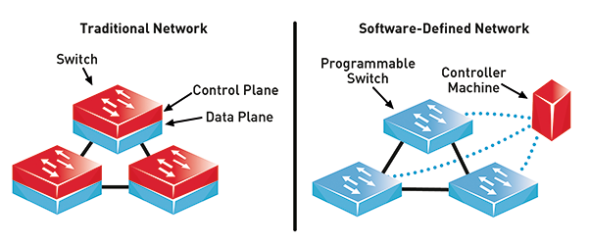
\includegraphics[width=6.5cm]{archivos/img/intro/sdn.png}
%     \caption{Paradigma en redes \glsentryshort{sdn}}
%     \label{sdnparadigma}
% \end{figure}

% Se considera como un punto de convergencia entre ambas tecnologías las redes 5G basadas fundamentalmente en \gls{sdn}, ya que prevén la incorporación de múltiples dispositivos \gls{iot}. Sin embargo, no todos los dispositivos \gls{iot} soportan una gestión basada en \gls{sdn} debido a las limitaciones que estos tienen en memoria, capacidad de procesamiento y  batería. Conforme el mundo de los dispositivos \gls{iot} avanza, las placas \gls{sbc} cada vez se hacen más potentes y de un tamaño más reducido, haciendo posible que éstas puedan ser incluidas como una pieza fundamental en proyectos \gls{iot} de alto rendimiento \cite{7501691}. \\

% \par

% Además, los sensores \gls{iot}, comúnmente conocidas como ``motas", continuamente se fabrican con más capacidad de procesamiento, memoria y batería con la finalidad de hacer frente a las nuevas redes de comunicaciones 5G \cite{capra2019edge}. Por todo ello,  se estima que la integración con las redes \gls{sdn} está cada vez más próxima. Generalmente, se están siguiendo estas vías de actuación:
% \begin{itemize}
%     \item \label{iot_integracionParcial}Realizar una integración parcial, haciendo uso de de dispositivos mediadores entre las motas y el core \gls{sdn}. Este dispositivo mediador, sería un dispositivo híbrido con interfaces inalámbricas y alámbricas para tener de acceso a la red \gls{sdn} \cite{7848825}.

%           \begin{figure}[h]
%               \centering
%               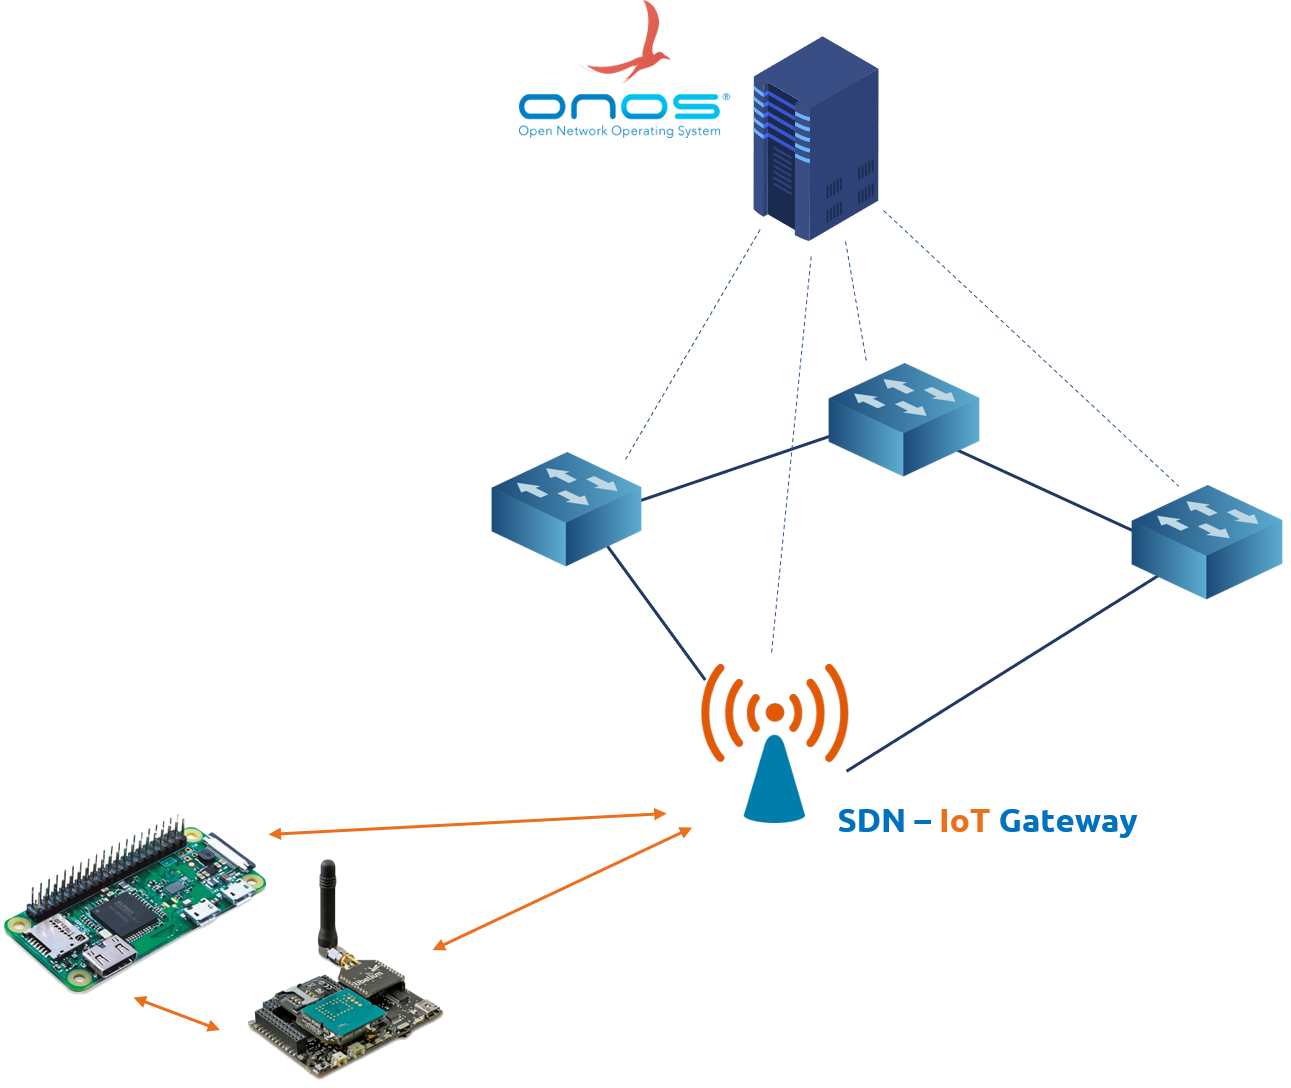
\includegraphics[width=10cm]{archivos/img/intro/sdn_iot.png}
%               \caption{Integración parcial de dispositivos \glsentryshort{iot} en el core \glsentryshort{sdn}}
%               \label{sdn_iot_parcial}
%           \end{figure}
%           Como se puede ver en la figura \ref{sdn_iot_parcial}, haciendo uso de un dispositivo mediador, este actuaría de pasarela o \textit{gateway} para las redes de sensores. De esta manera, se delega toda la carga de procesamiento y consumo de batería que supone integrar la interfaz de control \gls{sdn}. Además, se implementarían los distintos protocolos y estándares para comunicarse con los dispositivos \gls{iot}. Esta vía también ofrece otros aspectos positivos, entre los cuales se puede destacar, emplear el gateway como un traductor de protocolos \gls{iot} \cite{8470257}. Esto permitiría que distintos sensores que tuvieran implementados diferentes protocolos como, por ejemplo, \gls{ble}\footnote{Especificación del protocolo:  \url{https://www.bluetooth.com/specifications/}} y Zigbee\footnote{Protocolo de alto nivel basado en el estandar \gls{ieee} 802.15.4, especificación: \url{https://zigbeealliance.org/solution/zigbee/} }, pudieran interactuar entre sí a través del  gateway \gls{iot}.

%     \item \label{iot_integracionTotal}Realizar una integración total, como se puede apreciar en la figura \ref{sdn_iot_total}, donde el propio dispositivo \gls{iot} es capaz de co-existir en la red \gls{sdn}. Esta última vía es la más ambiciosa debido a que se requiere de hardware lo suficientemente potente para soportar la lógica \gls{sdn}, y de una tecnología que establezca su plano de datos de forma más eficiente posible para optimizar al máximo los recursos limitados del dispositivo.

%           \begin{figure}[ht]
%               \centering
%               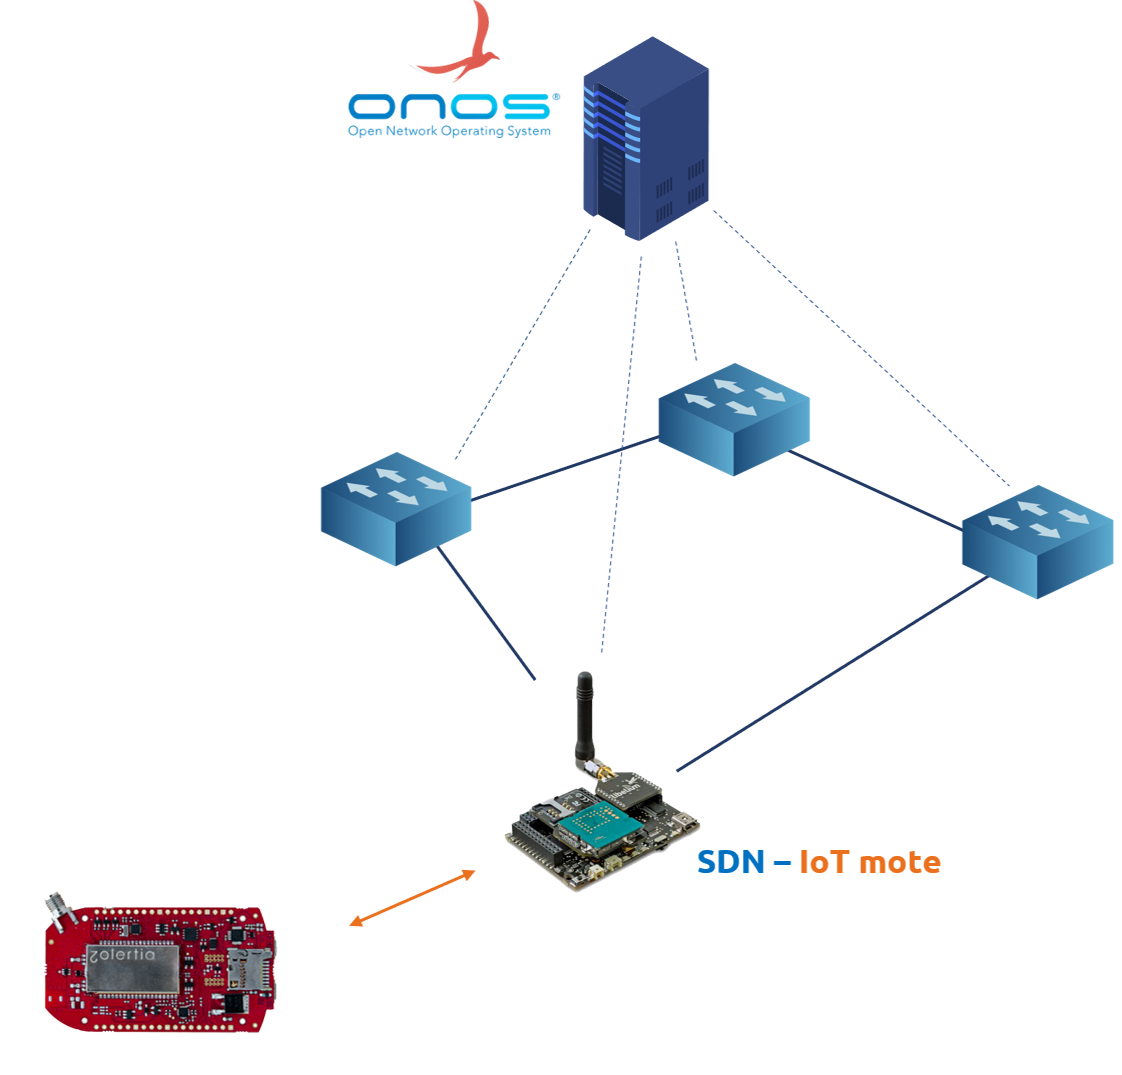
\includegraphics[width=10cm]{archivos/img/intro/sdn_iot_b.png}
%               \caption{Integración total de dispositivos \glsentryshort{iot} en el core \glsentryshort{sdn}}
%               \label{sdn_iot_total}
%           \end{figure}

% \end{itemize}



% \section{Tecnologías para la definición del datapath}



% En redes convencionales previas al concepto de \gls{sdn}, los nodos de la red tenían unificado un plano de control, \textit{Control plane}, donde se definía la lógica que dictaba como debía llevarse a cabo el \textit{forwarding} de los paquetes, y un plano de datos, \textit{Data plane}, el cual se puede implementar definiendo su datapath. Dicho datapath se compone de varios bloques de procesado para reenviar los paquetes. Con la llegada del paradigma de las redes \gls{sdn}, como se puede apreciar en la figura \ref{sdnparadigma}, los nodos clásicos de red verían como su plano de control sería delegado a una entidad llamada controlador. El controlador tendría una perspectiva global de toda la red en su conjunto pudiendo gestionarla de una manera más flexible y centralizada. \\
% \par
% En consecuencia, los nodos de la red estarían destinados a implementar un plano de datos, y una interfaz de control para ser configurados por el controlador mediante protocolos como, por ejemplo, OpenFlow\footnote{\url{https://www.opennetworking.org/software-defined-standards/specifications/}}. \\
% \par
% Por lo tanto, para ejecutar la integración de los dispositivos \gls{iot} en las redes \gls{sdn} se debe poder definir un datapath en dichos dispositivos y que estos posean una interfaz de control para ser configurados desde un hipotético controlador. Debido a esto, se requiere hacer uso de tecnologías que nos permitan definir el plano de datos de estos dispositivos. En este \gls{tfg}, se abordarán las siguientes tecnologías:

% \begin{itemize}
%     \item El lenguaje \textbf{P4}. Este lenguaje de alto nivel nos permite definir el procesado de los paquetes para un conjunto de arquitecturas. Dichas arquitecturas tienen su propia especificación. Con ello, se quiere conseguir que los programas P4 sean independientes del \textit{hardware} donde se ejecute \cite{2014p4}.

%     \item \textbf{\gls{xdp}}. Es un \textit{framework} programable y de alto rendimiento para el procesado de paquetes en el Kernel de Linux. El procesado de los paquetes se lleva a cabo en el punto más bajo de la pila de red de Linux, consiguiendo así añadir nuevas funcionalidades sin necesidad de modificar el propio Kernel. Además, el hecho de definir el procesado de paquetes casi en la propia interfaz, reporta un gran rendimiento ya que no es necesario atravesar toda la pila de protocolos, con todo lo que eso conlleva (reservas de memoria, reservas de memoria para metadatos, encolado de los paquetes, desencapsulado de cabeceras, análisis y tratamiento de cabeceras, etc) \cite{xdp1}.
% \end{itemize}



% \section{Objetivos}

% El objetivo de este proyecto es realizar un estudio y análisis de las tecnologías P4 y \gls{xdp} para la integración de dispositivos \gls{iot} en entornos \gls{sdn}. Como ya hemos introducido, con la llegada del \gls{iot}, la dimensión de las redes va a crecer exponencialmente. Por consiguiente, la complejidad de la administración de dichas redes va a suponer un gran desafío.  Los dispositivos \gls{iot} se podrán beneficiar de la integración con las redes \gls{sdn}, ya que éstas les reportarán la \textbf{flexibilidad} y \textbf{programabilidad} requerida para una correcta gestión y administración de cada elemento de la red. Para alcanzar dicho objetivo, se han planteado los siguientes puntos:

% \begin{itemize}
%     \item \textbf{Documentación y estudio}: Búsqueda y recolección de información, artículos y guías para tener
%           los conocimientos básicos necesarios sobre el estado del arte actual y de las tecnologías para definir el plano de datos. De esta forma, se podrá plantear los diseños y desarrollos más optimizados, de cara a favorecer las limitaciones impuestas por los dispositivos \gls{iot}.

%     \item \textbf{Planteamiento de casos de uso típicos y elección de escenarios}: Se hará un planteamiento de funcionalidades básicas, casos de uso, que una tecnología que define un datapath debe ser capaz de proveer. Además, se elegirán los escenarios y plataformas para desplegar dichos casos de uso.

%     \item  \textbf{Desarrollo de los casos de uso}: Se abordará el desarrollo de dichos casos de uso con ambas tecnologías (P4, \gls{xdp}) en los escenarios planteados. Se tratará que los escenarios donde se desplieguen los desarrollos sean lo más homogéneos posibles, para que los puntos fuertes y débiles de cada tecnología puedan ser esclarecidos.

%     \item \textbf{Evaluación y comprobación de funcionamiento}: Se comprobará el correcto funcionamiento de todos los casos de uso desarrollados y por último, se evaluará que tecnología es más idónea para definir el datapath de los dispositivos \gls{iot} en su integración en entornos \gls{sdn}.
% \end{itemize}


% \section{Estructura del \glsentryshort{tfg}}

% En esta sección se indica la estructura básica de este \gls{tfg}, haciendo un breve resumen de los aspectos más importantes y significativos de cada capítulo.


% \begin{description}
%     \item\textbf{Capítulo 1: Introducción}. Se hará una breve introducción de la motivación que ha originado la realización de este \gls{tfg}, así como una breve explicación de los aspectos generales y de los objetivos que se quieren alcanzar con el trabajo presentado.

%     \item\textbf{Capítulo 2: Estado del arte}. Se documentarán conceptos fundamentales en relación al proyecto, además de todas las diferentes herramientas que sean utilizadas. La motivación de este capítulo es la de establecer un marco teórico lo suficientemente consistente para abordar el análisis y el diseño de forma óptima, previo al desarrollo.

%     \item\textbf{Capítulo 3: Diseño y análisis de casos de uso}. Se debatirá y analizará que funcionalidades básicas deben tener las distintas tecnologías para definir el datapath. Para ello, se diseñarán distintos casos de uso para así demostrar la eficiencia de una tecnología sobre la otra en la integración de los dispositivos \gls{iot} en entornos \gls{sdn}.

%     \item\textbf{Capítulo 4: Desarrollo y evaluación de casos de uso}. Se describirá el desarrollo realizado, indicando las partes más importantes de cada caso de uso, ofreciendo al final de cada caso una evaluación de su funcionamiento.

%     \item\textbf{Capítulo 5: Conclusiones y trabajo futuro}. Se terminará la memoria con las conclusiones del trabajo realizado, y se presentarán las vías de trabajo futuro que tiene este proyecto.

%     \item[]\textbf{Bibliografía y referencias}. Se añadirán todos los artículos, libros, materiales consultados y empleados en la elaboración de esta memoria. Se seguirá el estilo de citación del \gls{ieee}, siguiendo las recomendaciones oficiales de la normativa sobre \gls{tfg}s de la \gls{uah}.

%     \item[]\textbf{Anexos}. Se incluirán todos los manuales de usuario e instalación que se consideren oportunos. De forma adicional, se añadirán las características técnicas del \textit{hardware} con el cual se ha desarrollado este \glsentryshort{tfg}. Por último, se hará un presupuesto que incluya el coste de mano de obra, material y gastos generales.

% \end{description}

%%%%%%%%%%%%%%%%%%%%%%%%%%%%%%%%%%%%%%%%%%%%%%%%%%%%%%%%%%%%%%%%%%%%%%%%%%%%%%%%%%%%%%%%%%%%%%%%%%%%